\section{Motivation}

% Motivação: contextualização do problema ou da necessidade que motivou o trabalho. Essa seção deve preparar o leitor para a <Pergunta da Pesquisa>

According to the World Health Organisation (WHO), there are at least 2.2 billion people with some visual impairment degree \cite{world2019world}. Hence there is a demand for assistive products in the world. This demand is driven by dissatisfaction with the current products since they are not practical, not portable, invasive or demandful to learn \cite{lozano2009electrotactile}.

This difficulty to use or to learn could be avoided if concepts from human factors, or ergonomics, were analyzed during the product's development, and these could be done using the proper methods. The early application of these methods and tests could be a game-changer for the success of the product's user experience \cite{wolf2019towards}.

Another tool that helps training and user efficiency is Virtual Reality (VR). VR can be used to create specific, immersive and interactive situations that could help the user to learn and train \cite{farrell2018learning} and the developers to create more efficient products.

Another strategy to improve the user experience is to bring the user closer to the development team {\textit{\large Adicionar mais coisa}}.

At the beginning of February 2022, about 400 million people had been diagnosed with COVID-19 around the world \cite{ourworldindata_cases}. Purposing to try to slow the rate at which the virus spread, WHO recommended strategies like wearing face masks, washing hands regularly, social distancing, avoiding touching surfaces and staying at home \cite{who_2020}.

Besides not having a desirable or easily adaptable guidance method, now BVI users' must avoid touching surfaces, an action that they depend on to perceive the environment, and keep distance from other people, a task that, besides being difficult to maintain, a BVI user is not used to since he/she depends on others to do their daily activities, like to cross the street \cite{jondani2021strategies}.

\section{Objectives}

 % Objetivo geral: é a proposta, contribuição ou a entrega que endereça a solução da pergunta da pesquisa

 The objectives of this master's thesis are to assess BVI users' using different guidance methods inside a Virtual Environment (VE) and to verify if non-BVI users have the same mental demand and situation awareness as BVI users when using assistive products to improve the development of new assistive solutions for BVI users.

 % Objetivos específicos: para a consecução do objetivo geral, foram identificados os seguintes objetivos específicos
 
 To reach this goal, the following questions must be answered:
 \begin{enumerate}
     \item Do BVI users feel present in the VE as if they were in the real world? \label{itm:obj_first}
     \item BVI users rely on audio cues and haptic feedback to guide. But does it rely more on one type of information than the other? \label{itm:obj_second}
     \item Do non-BVI users have the same demands and skills as BVI users when designing assistive products? \label{itm:obj_third}
 \end{enumerate}
 
 %\section{Reason}
 
 % Justificativa: há na literatura, certamente, vários trabalhos que endereçam o mesmo problema que você está pesquisando. Justifique porque você quer – ainda assim – pesquisar esse tema, posicionando o seu trabalho em relação aos demais autores.
 
 %We are entering the 4.0 Industry, where humans work beside robots that scan images in 3D, \textit{drive} autonomous cars and can print parts to assembly almost anything in the universe

\section{Resources and methods} 

%Recursos e métodos: para cada um dos objetivos específicos, foram definidos os seguintes recursos e métodos (...). Você tem que justificar que os objetivos específicos são factíveis

To answer all the questions and reach the goal mentioned above, the following resources were allocated:

\begin{itemize}
    \item To answer about the feeling of presence from BVI users in VE:
    \begin{itemize}
        \item HTC VIVE VR Head Mounted Device (HMD), as show in Figure \ref{fig:htc_vive};
        \item A guidance method evaluation questionnaires (See Appendix  \ref{sec:guidace_evaluation}) .
    \end{itemize}
    \item To answer if BVI users rely more on one type of information than the other and if non-BVI users can undergo the same situations as BVI users when using assistive products:
    \begin{itemize}
        \item Mental workload assessment, using:
            \begin{itemize}
                \item Physiological sensors (as show in Figure \ref{fig:sensores});
                \item NASA-TLX questionnaire (See Appendix  \ref{sec:nasa_tlx}).
            \end{itemize}
            \item Situation awareness assessment, using:
            \begin{itemize}
                \item SAGAT questionnaire (Adapted for this experiment. See Appendix \ref{sec:sagat}).
            \end{itemize}
    \end{itemize}
\end{itemize}

\begin{figure}[!htb]
    \begin{minipage}{.45\linewidth}
        \centering
        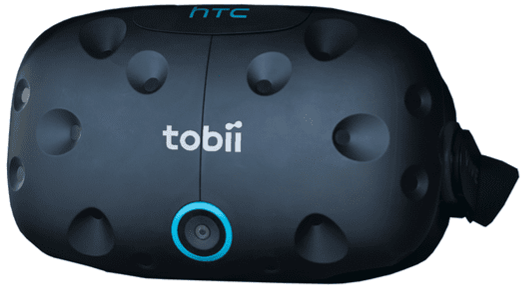
\includegraphics[width=\linewidth]{Introducao/VIVE.png}
        \vspace{1.2cm}
        \caption{VIVE HTC TOBII Virtual Reality Headset.}
        \label{fig:htc_vive}
    \end{minipage}
    \begin{minipage}{.1\linewidth}
        \hfill
    \end{minipage}
    \begin{minipage}{.45\linewidth}
        \centering
        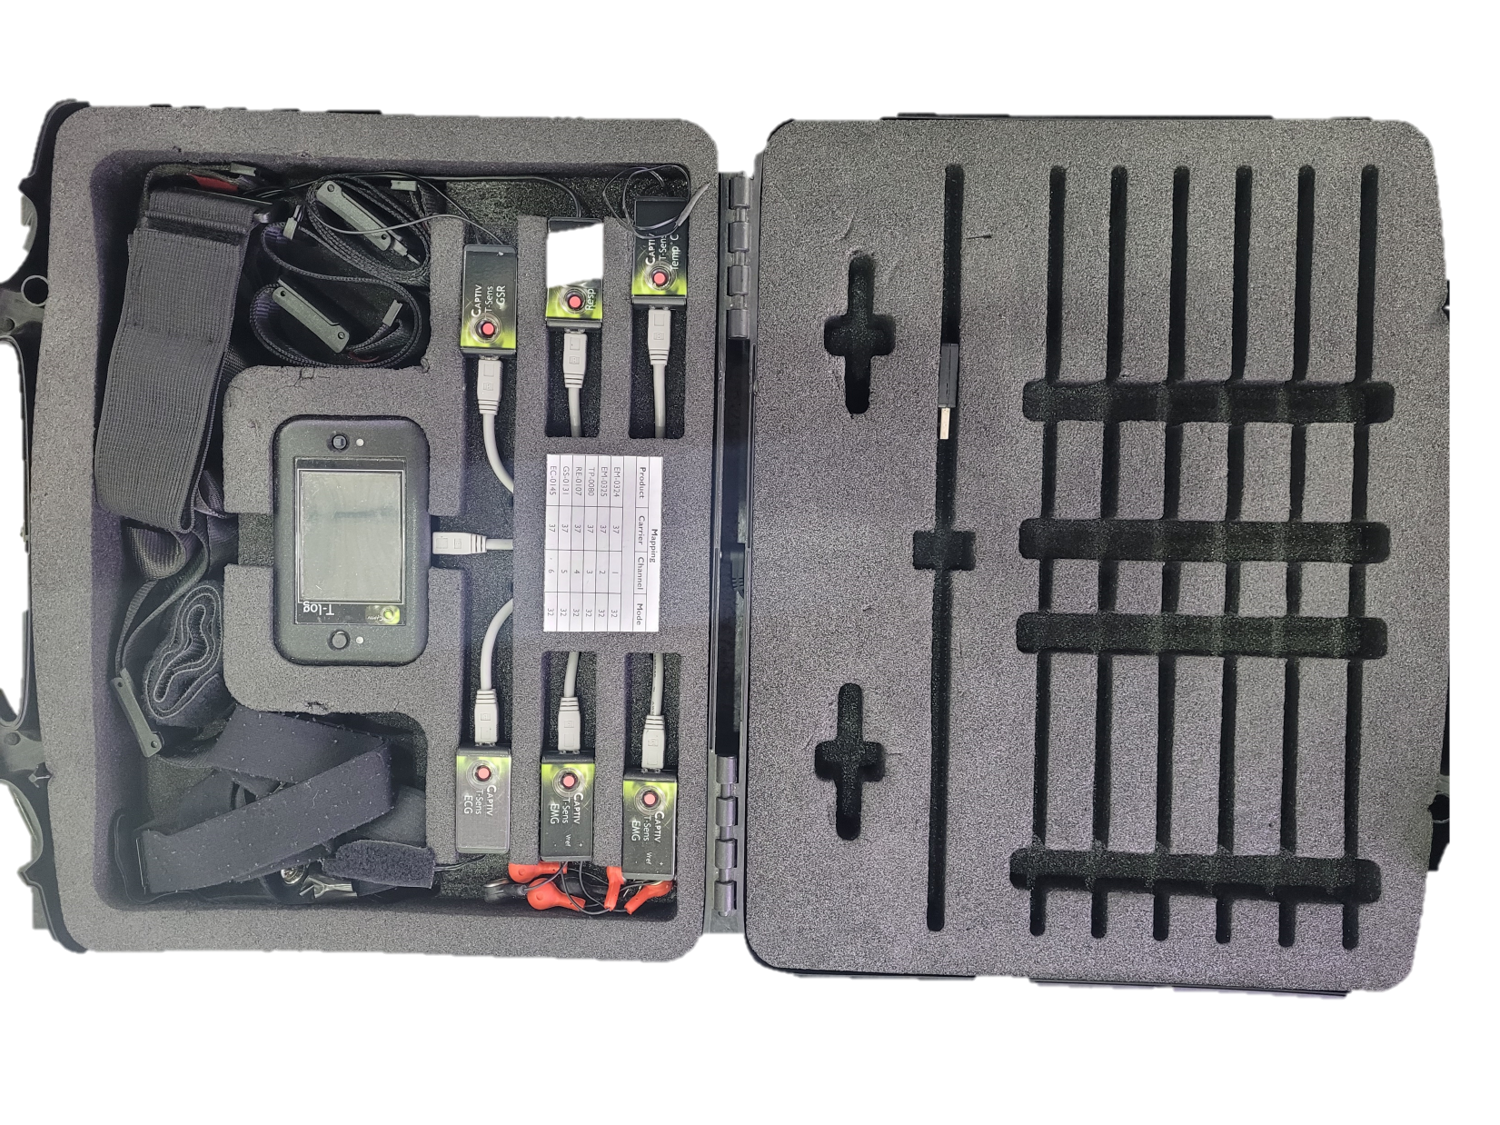
\includegraphics[width=\linewidth]{Introducao/sensores.png}
        \caption{Captive T-Sens sensors.}
        \label{fig:sensores}
    \end{minipage}
\end{figure}

\section{Research boundaries}

% Delimitação da pesquisa: é o recorte do seu trabalho

This experiment is not testing the usability of the guidance tools developed for it. These tools are only used here to help users and researchers compare the different feelings provoked by the information transmitted by it.

% Estrutura do texto

\section{Structure}

This master's thesis is organized in 8 different chapters and they the following:

\begin{itemize}
    \item {\large\textbf{{~\nameref{ch:introducao}}}}
        
        It's the current chapter of this master's thesis
    
    \item {\large\textbf{{~\nameref{ch:fundamentacao}}}}
    
        This chapter explores the mains concepts that are needed to fully understand this experiment. These concepts are:
        
        \begin{itemize}
            \item {~\nameref{sec:human_factors}};
            \item {~\nameref{sec:mental_workload}};
            \item {~\nameref{subsec:task_performance}};
            \item {~\nameref{subsec:physiological_measures}};
            \item {~\nameref{subsec:subjective_measures}}.
            \item {~\nameref{sec:situation_awareness}};
            \item {~\nameref{sec:extended_reality}};
            \item {~\nameref{subsec:virtual_reality}};
            \item {~\nameref{sec:co_design}}.
            
        \end{itemize}
    
    \item {\large\textbf{{~\nameref{ch:revisao}}}}
    
        During this chapter, related articles, i.e articles that involve applications of:
        \begin{itemize}
            \item VR;
            \item BVI users;
            \item Human factors.
        \end{itemize}
        All these articles have some relevance to the current experiment.
    
    \item {\large\textbf{{~\nameref{ch:metodologia}}}}
    
        Within this chapter, the method used to reach the goals presented above will be explained.
    
    \item {\large\textbf{{~\nameref{ch:cenario}}}}
        
        This chapter is dedicated to explaining the steps that were taken to design the scene used during the experiment
        
    \item {\large\textbf{{~\nameref{ch:cinto}}}}
        
        In this chapter, the process of coding and assembly of the haptic belt is explained.
        
    \item {\large\textbf{{~\nameref{ch:resultados}}}}
    
        One of the main chapters of this work. Here are presented and discussed all the gathered results and data
    
    \item {\large\textbf{{~\nameref{ch:conclusao}}}}
    
        Finally, which goals were reached and which were not and why they were not.
    
\end{itemize}


%\subsection{~\nameref{ch:introducao}}
%
%%\emph{O capítulo 1 contém a introdução do trabalho, onde são expostos o objetivo, a motivação do %mesmo, a descrição do sistema e a formulação do problema com a nomenclatura utilizada; além de uma %revisão bibliográfica da literatura relacionada ao tema do trabalho.}
%
%\subsection{~\nameref{ch:revisao}}
%
%%\emph{No capítulo 2 apresentamos a modelagem dinâmica de um manipulador subatuado e o conceito de %índice de acoplamento para medir o acoplamento dinâmico entre as juntas ativas e passivas. Este %índice é utilizado para a análise e projeto de uma metodologia de controle subótimo do %manipulador.}
%
%In this chapter 
%
%
%\subsection{~\nameref{ch:fundamentacao}}
%
%\subsection{~\nameref{ch:metodologia}}
%
%\emph{O capítulo 3 apresenta o controle subótimo de manipuladores através de redundância de %atuação. Descreve-se a técnica de controle ponto a ponto de manipuladores subatuados. A seguir %mostramos  a linearização destes por realimentação, cujo efeito é linearizar e desacoplar o sistema %não linear. Finalmente é proposta uma sequência de controle subótimo local das juntas passivas %visando a minimização de certos critérios como torque, velocidade e em particular a energia %consumida pelo sistema. Este é de fato o tema principal deste mestrado.}
%
%
%\subsection{~\nameref{ch:cenario}}
%
%\subsection{~\nameref{ch:cinto}}
%
%\subsection{~\nameref{ch:resultados}}
%
%\emph{É também apresentado no capítulo 4 um resumo do projeto de controladores  $H_{2}$ e %$H_{\infty}$, cuja principal vantagem é a robustez na presença de incertezas paramétricas e %distúrbios externos.}
%
%\subsection{~\nameref{ch:conclusao}}
%
%\emph{No capítulo 5 são apresentadas as conclusões do trabalho.}
%
%